This section extends upon the fundamentals mentioned in the Turtlenet (TN)
general section.

\section{Creating an Account}
The 'General' chapter only briefly mentions creating an account so to make this
section complete as a 'go-to' resource for users it will also be mentioned here
too.

This is where your private communications begin.  Therefore it is important that
this is done correctly otherwise you can't bolster your privacy with our client.

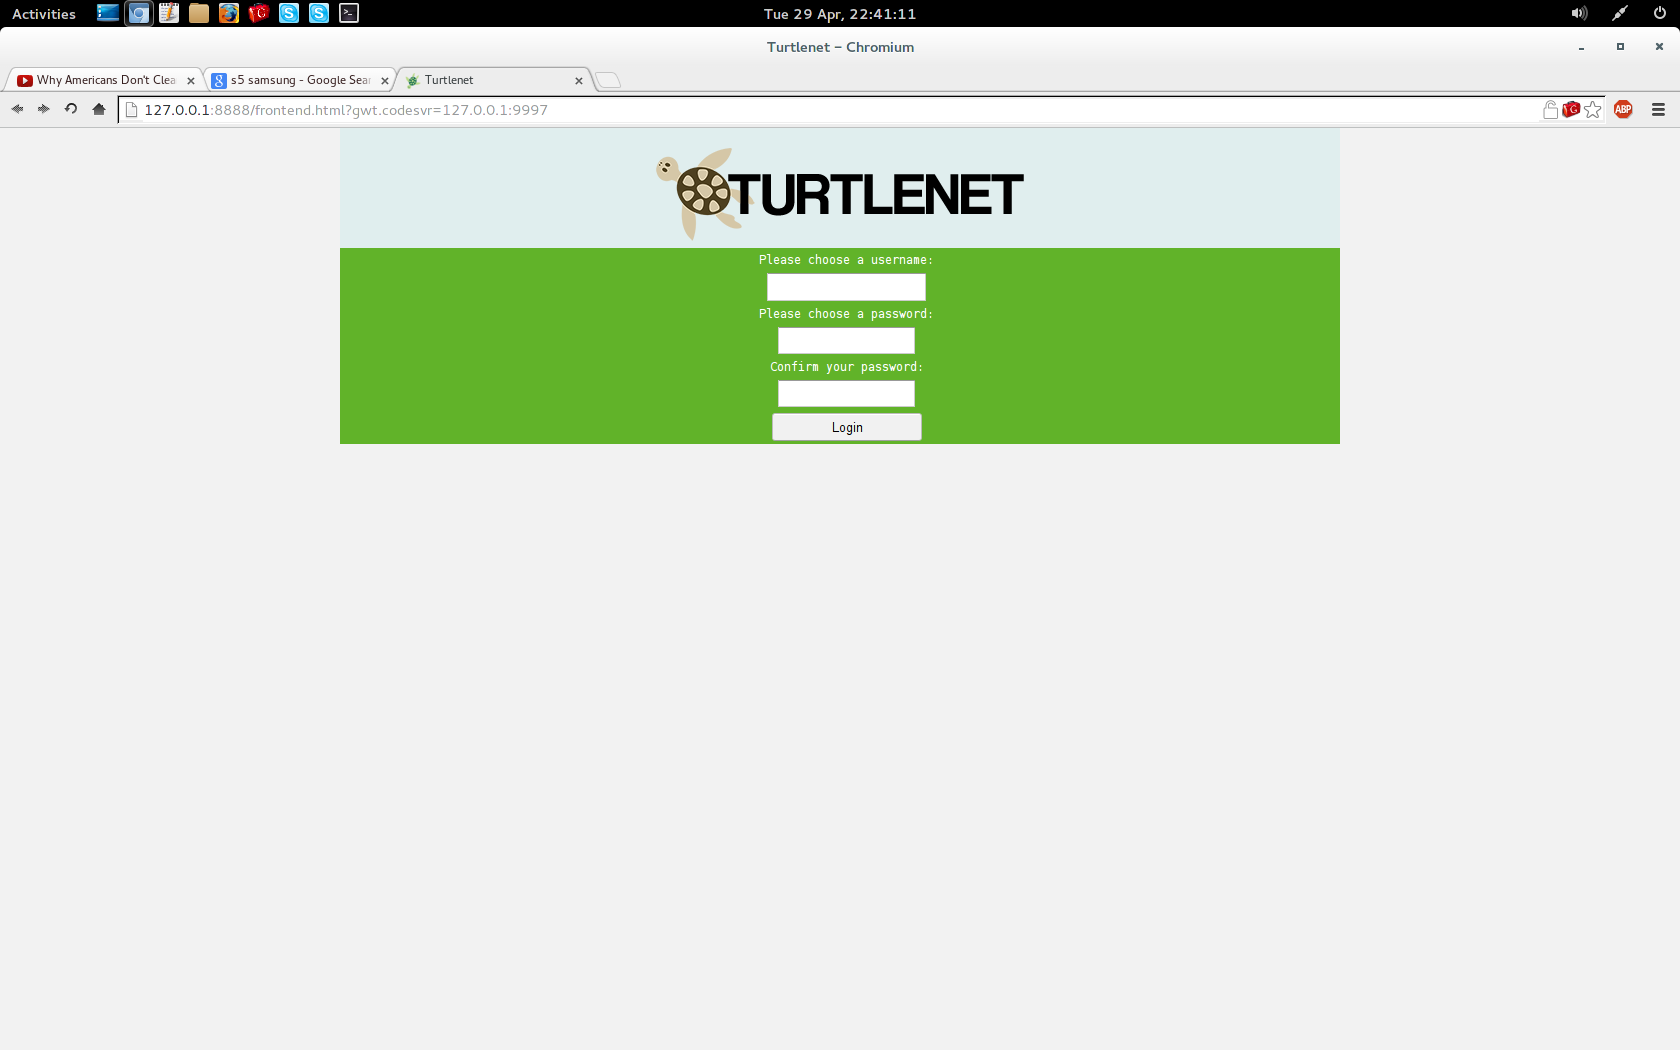
\includegraphics[scale=0.2]{../Screenshots/Screenshot from 2014-04-29 22-41-11}

This image shows the account creation page, which you should see when you run 
the client for the first time on your computer.  From the top there are three
text boxes:
\begin{itemize}
\item a Username box
\item a Password box
\item a Confirmation box
\end{itemize}

You fill in each of the fields with the required information which will be the
following:
\begin{itemize}
\item The Username box should be filled in with your user name.  This is what
      other users would call you when posting messages.  This should be 
      something that represents you, but should not link to you outside of
      Turtlenet.  Simply, your Turtlenet user name should not be the same as
      any other user name you use on the internet.  Can't improve anonymity if
      you use the same name around the internet.
\item The Password is important as it is the only form of validation for logging
      into Turtlenet.  Therefore it should be easy to remember but difficult for
      anyone else to crack.  A good method for coming up with new passwords is
      to use four or five words, like a phrase you use.  An example would be
      'ThisIsTurtlenetzPassword'.  This is better and easier to remember than
      what is usually suggested which is a shorter password with numbers in
      them: 'P@ssw0rd'.  Of course, it depends on who is remembering the
      password so choose your own method if either option mentioned feels
      uncomfortable for you.
\item The Confirmation box is where you type the password you defined in the
      previous box.  Because of this, they should match, and must if the account
      creation is to be successful.  The easiest way of thinking about this box
      is that it is giving you the practice of inputting your password while it
      is still fresh in your mind, to help you remember for later on.
\end{itemize}

By filling in these text boxes with the kind of information mentioned in this
section, you can then click the button underneath these boxes to create your
account.  If successful, the password prompt screen should appear and you can
move onto logging into Turtlenet to begin the communicative fun!

\section{Logging into Turtlenet}
Logging into the Turtlenet client is as simple as using the password that you
had used to create your account, as it is your primary method of informing the
system of who you are.  Please understand that whilst the password is a way of
proving that you are 'you,' other users will not know your password, or even
anything you post until you link them your public key, which will be covered
later in this chapter.

\includegraphics[scale=0.2]{../Screenshots/Screenshot from 2014-04-29 22-24-59}

The screen shot shows the initial page you might see once you have created an
account.  Enter your password into the white text box above the 'Login' button
and if the password is correct, you would have logged in.

\section{Navigating around the Turtlenet client}
Getting around the client's various areas is important in order to make the most
of the functionality provided by Turtlenet.  This is why all of the main
segments are provided as buttons at the top of the interface:

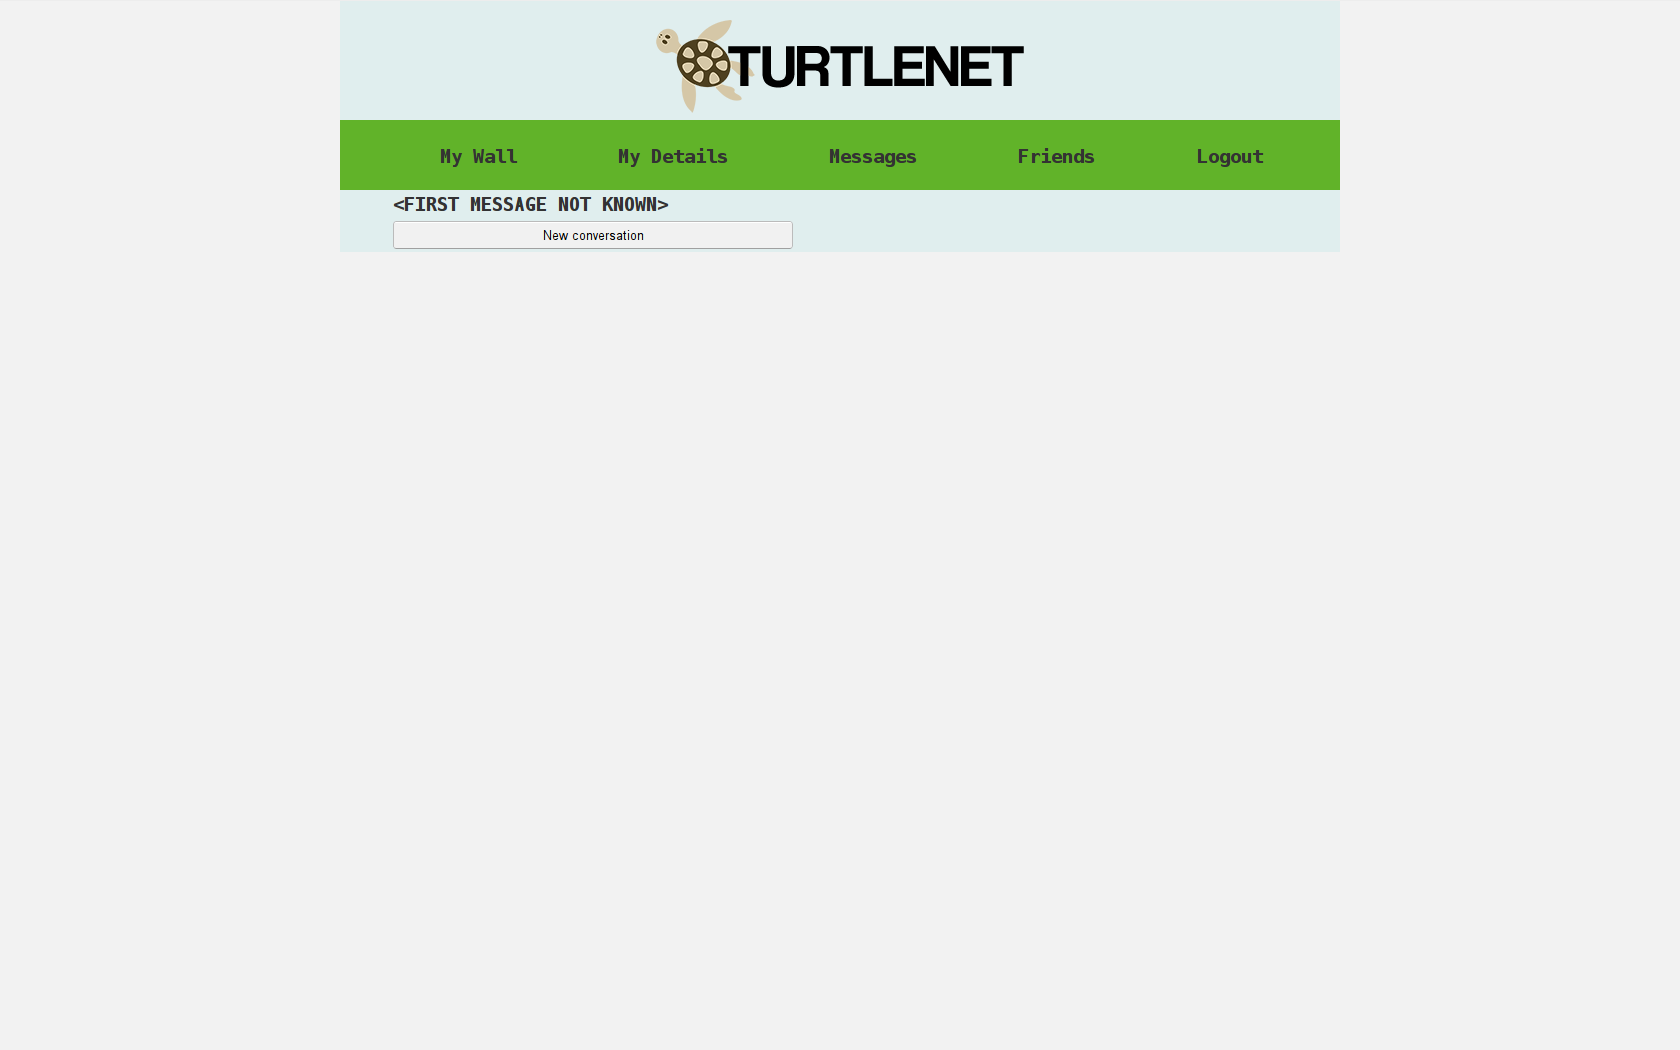
\includegraphics[scale=0.2]{../Screenshots/Screenshot from 2014-04-29 22-31-38}

The image shows that there are several main sections to the client - The wall,
the user's details, messages between the user and other people, friends that the
user has linked with and finally the function to logout.  Click the
corresponding button to get to the area you wish to view.  The following
chapters will go through each section from right to left, as it is important to
obtain other users that can read what you post.

\section{Logging out}
For when you decide that you want to leave the safety of Turtlenet and work on
other things, or you simply need to be away for a while and want to be sure that
no one is using your account, you will want to log off.  It is as painless as
clicking the 'log off' button found at the top right of every page.  Doing so
will take you to the login screen (the one with just the password box and login
button).  Of course, we wish you good fortune until you come and join us again
at Turtlenet.

\section{Getting and Making Friends on Turtlenet}
Part of the philosophy of Turtlenet is to encrypt the messages that you send so
that only the intended recipients can read them with any understanding.  These
people are known as your 'friends' on Turtlenet.  In order to make any use of
Turtlenet you need to add friends.  You do this by exchanging 'public keys' with
another user.  Turtlenet uses Asymmetric relationships - this means that you may
have some people as friends but they might not have you as a friend.  Therefore
you might understand what people have typed but they might not be reciprocated.
If this doesn't make sense at the moment, the following chapters will help.

\subsection{The 'Getting'}
In order to get public keys from other users, they need to pass the information
to you in some other format - it is near, if not fully, impossible to pass the
key through Turtlenet so you need to agree to some other form of communication
until Turtlenet is set up for both you and your soon-to-be TN-friends.  In an
internet based age, the most secure, and ironic, way of getting the key off of
your friend would use a method that does not use the internet, such as a text
message or a phone call - even standard mail would suffice and be more secure
than an internet equivalent.

Once you have the public key off of your friend, you will want to proceed to the
'friends' section of the Turtlenet client, by clicking the button near the top
which has 'Friends' written upon it.  You should either see the following or
something to it's effect:

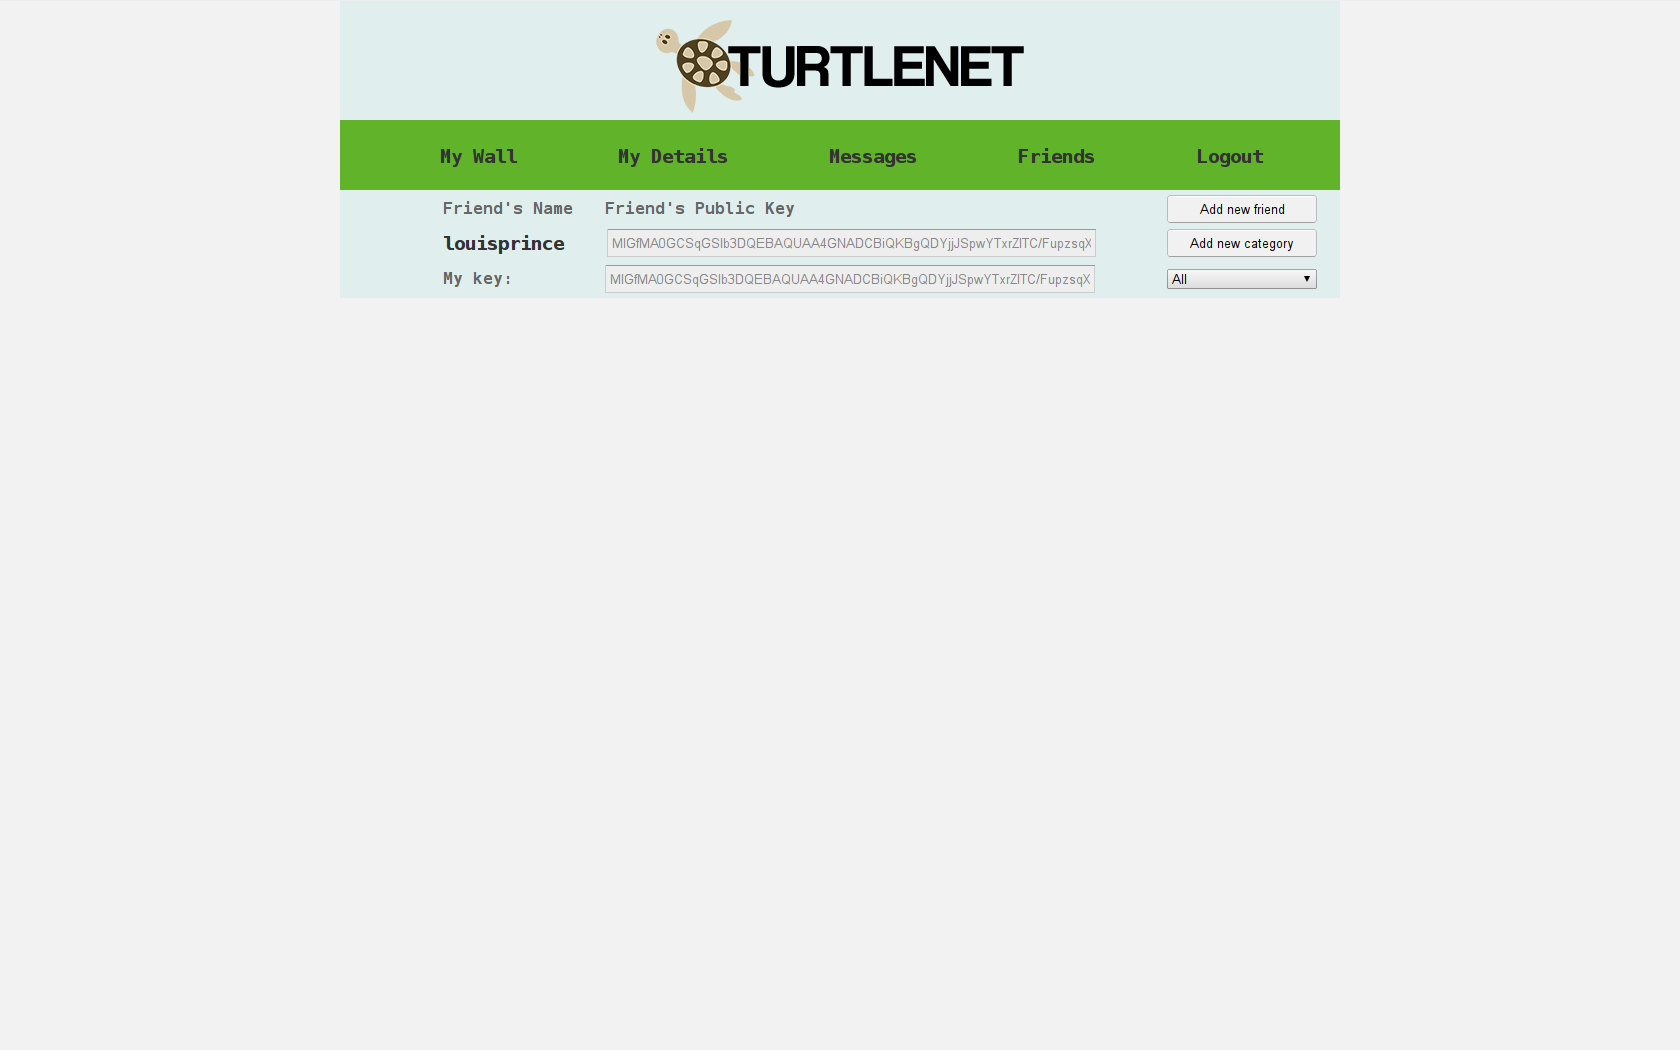
\includegraphics[scale=0.2]{../Screenshots/Screenshot from 2014-04-29 22-31-10}

As you can see, there is 'My Key' which will be used by you to allow others to
send you messages but that will be explained in the next chapter.  

